%%%%%%%%%%%%%%%%%%%%%%%%%%%%%%%%%
% baposter Landscape Poster
% LaTeX Template
% Version 1.0 (15/5/13)
%
% Created by:
% Brian Amberg (baposter@brian-amberg.de)
%
% This template has been downloaded from:
% http://www.LaTeXTemplates.com
%
% License:
% CC BY-NC-SA 3.0 (http://creativecommons.org/licenses/by-nc-sa/3.0/)
%
%%%%%%%%%%%%%%%%%%%%%%%%%%%%%%%%%%%%%%%%%

%----------------------------------------------------------------------------------------
%	PACKAGES AND OTHER DOCUMENT CONFIGURATIONS
%----------------------------------------------------------------------------------------

\documentclass[a0paper,portrait,fontscale=0.3, margin=2cm]{baposter}

\usepackage[utf8]{inputenc}
\usepackage[font=normalsize,labelfont=bf]{caption} % Required for specifying captions to tables and figures
\captionsetup{justification=centering}
\usepackage{booktabs} % Horizontal rules in tables
\usepackage{lmodern}
\usepackage{relsize} % Used for making text smaller in some places

% Other packages
\usepackage{tabularx}
\def\tabularxcolumn#1{m{#1}}
\def\imagetop#1{\vtop{\null\hbox{#1}}}
\usepackage{adjustbox}
\usepackage{subfig}
\usepackage{floatrow} % sidecapfloat
\usepackage{setspace}
\usepackage{xspace}
\usepackage{noReferences}
\usepackage{caption}
\usepackage{tikz}
\usepackage[customcolors]{hf-tikz}
%\usepackage{subcaption}
\usepackage{epsf}
\usepackage{amsmath}
\usepackage{mathtools}
\usepackage{amssymb}
\usepackage{amsfonts}
\usepackage{amsthm}
\usepackage{dsfont}
\usepackage{enumitem}
\usepackage{float}
\usepackage{cases}
\usepackage{verbatim}
\usepackage{array}
\usepackage{graphicx}
\usepackage{graphics}
\usepackage{multirow}
\usepackage{listings}
%\usepackage[authoryear]{natbib}
\usepackage{authblk}
\usepackage[linesnumbered,ruled,vlined]{algorithm2e}
\usepackage{eqparbox}
\usepackage{xcolor}
\usepackage[backend=biber, citestyle=authoryear, maxcitenames=2, maxbibnames=2]{biblatex}
\usepackage{lipsum}
\usepackage{svg}
\usepackage{cleveref}
\usepackage{tikz}
\usepackage{xspace}
\usetikzlibrary{arrows,automata}
\usepackage{array, makecell}
\usepackage{pgfplots}
\usetikzlibrary{intersections}


\bibliography{../budgeted_rl.bib}


% Arrows
\newcommand{\incarrow}{{
\includegraphics[height=0.7\baselineskip]{./img/arrow_list}}}
\newcommand{\xmark}{\ding{55}}%

% Colors for slides
\definecolor{rouge1}{RGB}{226,0,38}  % red P
\definecolor{orange1}{RGB}{243,154,38}  % orange P
\definecolor{jaune}{RGB}{254,205,27}  % jaune P
\definecolor{blanc}{RGB}{255,255,255} % blanc P

\definecolor{rouge2}{RGB}{230,68,57}  % red S
\definecolor{orange2}{RGB}{236,117,40}  % orange S
\definecolor{taupe}{RGB}{134,113,127} % taupe S
\definecolor{gris}{RGB}{91,94,111} % gris S
\definecolor{bleu1}{RGB}{38,109,131} % bleu S
\definecolor{bleu2}{RGB}{28,50,114} % bleu S
\definecolor{vert1}{RGB}{133,146,66} % vert S
\definecolor{vert3}{RGB}{20,200,66} % vert S
\definecolor{vert2}{RGB}{157,193,7} % vert S
\definecolor{vertsolarized}{RGB}{211,233,219} % vert S
\definecolor{darkyellow}{RGB}{233,165,0}  % orange S
\definecolor{lightgray}{rgb}{0.9,0.9,0.9}
\definecolor{darkgray}{rgb}{0.6,0.6,0.6}

% Highlights for slides
\newcommand{\rcol}[1]{\textcolor{red}{\textit{#1}}}
%\newcommand{\eqrcol}[1]{\textcolor{red}{#1}}
%\newcommand{\eqrcolb}[1]{\textcolor{red}{\boldsymbol{#1}}}
\newcommand{\gcol}[1]{\textcolor{vert3}{\textit{#1}}}
%\newcommand{\eqgcol}[1]{\textcolor{vert3}{#1}}
%\newcommand{\eqgcolb}[1]{\textcolor{vert3}{\boldsymbol{#1}}}
\newcommand{\blcol}[1]{\textcolor{blue}{\textit{#1}}}
%\newcommand{\eqbcol}[1]{\textcolor{blue}{#1}}
%\newcommand{\eqbcolb}[1]{\textcolor{blue}{\boldsymbol{#1}}}
\newcommand{\ycol}[1]{\textcolor{darkyellow}{\textit{#1}}}
\newcommand{\eqycol}[1]{\textcolor{darkyellow}{#1}}

\newcommand{\rcolbm}[1]{$\textcolor{red}{\boldsymbol{#1}}$}
\newcommand{\rcolb}[1]{\textcolor{red}{\textit{\textbf{#1}}}}
\newcommand{\gcolb}[1]{\textcolor{vert3}{\textit{\textbf{#1}}}}
\newcommand{\bcolb}[1]{\textcolor{blue}{\textit{\textbf{#1}}}}
\newcommand{\ycolb}[1]{\textcolor{darkyellow}{\textit{\textbf{#1}}}}

% Colored boxes
\newcounter{ColoredBoxesCounter}
\newcommand{\highlightnew}[3][(0.0,-0.1)(-0.0,0.3)]{
\hfsetfillcolor{#2!20}
\hfsetbordercolor{#2!80}
\tikzmarkin{\theColoredBoxesCounter}#1
#3
\tikzmarkend{\theColoredBoxesCounter}
\stepcounter{ColoredBoxesCounter}
}

\newcommand{\highlight}[2][yellow]{\mathchoice%
{\colorbox{#1}{$\displaystyle#2$}}%
{\colorbox{#1}{$\textstyle#2$}}%
{\colorbox{#1}{$\scriptstyle#2$}}%
{\colorbox{#1}{$\scriptscriptstyle#2$}}}%

\newcommand{\eqrcol}[1]{\highlight[red!20]{#1}}
\newcommand{\eqrcolb}[1]{\highlight[red!20]{\boldsymbol{#1}}}
\newcommand{\eqgcol}[1]{\highlight[vert3!20]{#1}}
\newcommand{\eqgcolb}[1]{\highlight[vert3!20]{\boldsymbol{#1}}}
\newcommand{\eqbcol}[1]{\highlight[blue!20]{#1}}
\newcommand{\eqbcolb}[1]{\highlight[blue!20]{\boldsymbol{#1}}}

\colorlet{redp}{red!20} % vert S
\colorlet{greenp}{vert3!20} % vert S
\colorlet{bluep}{blue!20} % vert S
\colorlet{yellowp}{yellow!20} % vert S

\newcommand{\hl}[3][\fboxsep1pt]{{#1\colorbox{#2}{#3}}}%

\newcommand{\hlr}[1]{\hl{redp}{#1}}
\newcommand{\hlg}[1]{\hl{greenp}{#1}}
\newcommand{\hlb}[1]{\hl{bluep}{#1}}
\newcommand{\hly}[1]{\hl{yellowp}{#1}}

\newcommand{\hler}[1]{\hl[\fboxsep0pt]{redp}{$\displaystyle {#1}$}}
\newcommand{\hleg}[1]{\hl[\fboxsep0pt]{greenp}{$\displaystyle {#1}$}}
\newcommand{\hleb}[1]{\hl[\fboxsep0pt]{bluep}{$\displaystyle {#1}$}}

\newcommand{\hlbr}[1]{\hl[\fboxsep0pt]{redp}{$\displaystyle \mathbf{#1}$}}
\newcommand{\hlbg}[1]{\hl[\fboxsep0pt]{greenp}{$\displaystyle \mathbf{#1}$}}
\newcommand{\hlbb}[1]{\hl[\fboxsep0pt]{bluep}{$\displaystyle \mathbf{#1}$}}

\newcommand{\vph}{\vphantom{A_A^A}}

% Box for algorithms
\newlength{\minipagewidth}
\newlength{\minipagewidthx}
\setlength{\minipagewidth}{\columnwidth}
\setlength{\minipagewidthx}{\columnwidth}
\setlength{\fboxsep}{0.1mm}
\addtolength{\minipagewidth}{-\fboxrule}
\addtolength{\minipagewidth}{-\fboxrule}
\addtolength{\minipagewidth}{-\fboxsep}
\addtolength{\minipagewidth}{-\fboxsep}
\addtolength{\minipagewidthx}{+\fboxsep}
\newcommand{\bookbox}[1]{\small
\par\medskip\noindent
\framebox[\columnwidth]{
\begin{minipage}{\minipagewidth} {#1} \end{minipage} } \par\medskip }

\newcommand{\bookboxx}[1]{
\par\medskip\noindent
\framebox[\columnwidth]{
\begin{minipage}[t]{0.98\columnwidth} {\par\smallskip#1\par\smallskip} \end{minipage} } \par\medskip }


\usepackage{array}
\newcolumntype{L}[1]{>{\raggedright\let\newline\\\arraybackslash\hspace{-3.1cm}}m{#1}}
\newcolumntype{C}[1]{>{\centering\let\newline\\\arraybackslash\hspace{135pt}}m{#1}}
\newcolumntype{R}[1]{>{\raggedleft\let\newline\\\arraybackslash\hspace{-10pt}}m{#1}}

\newenvironment{myfont}{\fontfamily{kurier}\selectfont}{\par}
\newenvironment{myfont2}{\fontfamily{epigrafica}\selectfont}{\par}

% Border color of content boxes
\definecolor{bordercol}{RGB}{0,0,0}  %black
% Background color for the header in the content boxes (left side)
\definecolor{headercol1}{RGB}{200,0,0}        %red:RGB {200,0,0} 
% Background color for the header in the content boxes (right side) 
\definecolor{headercol2}{rgb}{1.0,0.49,0.0}        %orange:rgb {1.0,0.49,0.0}
% Text color for the header text in the content boxes
\definecolor{headerfontcol}{rgb}{1,1,1}  %white
% Background color for the content in the boxes
\definecolor{boxcolor}{rgb}{1,1,1} 

\definecolor{lightblue}{rgb}{0.145,0.6666,1}

\newsavebox\CBox
\newcommand\hcancel[2][0.5pt]{%
  \ifmmode\sbox\CBox{$#2$}\else\sbox\CBox{#2}\fi%
  \makebox[0pt][l]{\usebox\CBox}%  
  \rule[0.3\ht\CBox-#1/2]{\wd\CBox}{#1}}



%%%%%%%%%%%%%%%%%%%%%%%%%%%%
% Paper dependent stuff    %
%%%%%%%%%%%%%%%%%%%%%%%%%%%%

\newcommand{\MLPC}{\texttt{MLP/Coordinates}\xspace}
\newcommand{\MLPG}{\texttt{MLP/Grid}\xspace}
\newcommand{\EgoAtt}{\texttt{Ego-Attention}\xspace}


%%%%%%%%%%%%%%%%%%%%%%%%%%%%
% Aesthetics               %
% over-underline, hat, bold%
%%%%%%%%%%%%%%%%%%%%%%%%%%%%

\newcommand{\eps}{\varepsilon}
\newcommand{\vareps}{\varepsilon}
\renewcommand{\epsilon}{\varepsilon}
%\renewcommand{\hat}{\widehat}
\renewcommand{\tilde}{\widetilde}
\renewcommand{\bar}{\overline}

\newcommand*{\MyDef}{\mathrm{\tiny def}}
\newcommand*{\eqdefU}{\ensuremath{\mathop{\overset{\MyDef}{=}}}}% Unscaled version



\def\:#1{\protect \ifmmode {\mathbf{#1}} \else {\textbf{#1}} \fi}
\newcommand{\CommaBin}{\mathbin{\raisebox{0.5ex}{,}}}

\newcommand{\wt}[1]{\widetilde{#1}}
\newcommand{\wh}[1]{\widehat{#1}}
\newcommand{\wo}[1]{\overline{#1}}
\newcommand{\wb}[1]{\overline{#1}}

% bf and bm missing due to conflict!!
\newcommand{\bsym}[1]{\mathbf{#1}}
\newcommand{\bzero}{\mathbf{0}}
\newcommand{\ba}{\mathbf{a}}
\newcommand{\bb}{\mathbf{b}}
\newcommand{\bc}{\mathbf{c}}
\newcommand{\bd}{\mathbf{d}}
\newcommand{\be}{\mathbf{e}}
\newcommand{\bg}{\mathbf{g}}
\newcommand{\bh}{\mathbf{h}}
\newcommand{\bi}{\mathbf{i}}
\newcommand{\bj}{\mathbf{j}}
\newcommand{\bk}{\mathbf{k}}
\newcommand{\bl}{\mathbf{l}}
\newcommand{\bn}{\mathbf{n}}
\newcommand{\bo}{\mathbf{o}}
\newcommand{\bp}{\mathbf{p}}
\newcommand{\bq}{\mathbf{q}}
\newcommand{\br}{\mathbf{r}}
\newcommand{\bs}{\mathbf{s}}
\newcommand{\bt}{\mathbf{t}}
\newcommand{\bu}{\mathbf{u}}
\newcommand{\bv}{\mathbf{v}}
\newcommand{\bw}{\mathbf{w}}
\newcommand{\bx}{\mathbf{x}}
\newcommand{\by}{\mathbf{y}}
\newcommand{\bz}{\mathbf{z}}

\newcommand{\bA}{\mathbf{A}}
\newcommand{\bB}{\mathbf{B}}
\newcommand{\bC}{\mathbf{C}}
\newcommand{\bD}{\mathbf{D}}
\newcommand{\bE}{\mathbf{E}}
\newcommand{\bF}{\mathbf{F}}
\newcommand{\bG}{\mathbf{G}}
\newcommand{\bH}{\mathbf{H}}
\newcommand{\bI}{\mathbf{I}}
\newcommand{\bJ}{\mathbf{J}}
\newcommand{\bK}{\mathbf{K}}
\newcommand{\bL}{\mathbf{L}}
\newcommand{\bM}{\mathbf{M}}
\newcommand{\bN}{\mathbf{N}}
\newcommand{\bO}{\mathbf{O}}
\newcommand{\bP}{\mathbf{P}}
\newcommand{\bQ}{\mathbf{Q}}
\newcommand{\bR}{\mathbf{R}}
\newcommand{\bS}{\mathbf{S}}
\newcommand{\bT}{\mathbf{T}}
\newcommand{\bU}{\mathbf{U}}
\newcommand{\bV}{\mathbf{V}}
\newcommand{\bW}{\mathbf{W}}
\newcommand{\bX}{\mathbf{X}}
\newcommand{\bY}{\mathbf{Y}}
\newcommand{\bZ}{\mathbf{Z}}

% calligraphic
\newcommand{\cf}{\mathcal{f}}
\newcommand{\cA}{\mathcal{A}}
\newcommand{\cB}{\mathcal{B}}
\newcommand{\cC}{\mathcal{C}}
\newcommand{\cD}{\mathcal{D}}
\newcommand{\cE}{\mathcal{E}}
\newcommand{\cF}{\mathcal{F}}
\newcommand{\cG}{\mathcal{G}}
\newcommand{\cH}{\mathcal{H}}
\newcommand{\cI}{\mathcal{I}}
\newcommand{\cJ}{\mathcal{J}}
\newcommand{\cK}{\mathcal{K}}
\newcommand{\cL}{\mathcal{L}}
\newcommand{\cM}{\mathcal{M}}
\newcommand{\cN}{\mathcal{N}}
\newcommand{\cO}{\mathcal{O}}
\newcommand{\cP}{\mathcal{P}}
\newcommand{\cQ}{\mathcal{Q}}
\newcommand{\cR}{\mathcal{R}}
\newcommand{\cS}{\mathcal{S}}
\newcommand{\cT}{\mathcal{T}}
\newcommand{\cU}{\mathcal{U}}
\newcommand{\cV}{\mathcal{V}}
\newcommand{\cW}{\mathcal{W}}
\newcommand{\cX}{\mathcal{X}}
\newcommand{\cY}{\mathcal{Y}}
\newcommand{\cZ}{\mathcal{Z}}

%%%%%%%%%%%%%%%%%%%%%%%%%%%%
% Math jargon              %
%%%%%%%%%%%%%%%%%%%%%%%%%%%%
\newcommand{\wrt}{w.r.t.\xspace}
\newcommand{\defeq}{\stackrel{\mathclap{\normalfont\mbox{\tiny def}}}{=}}
\newcommand{\maxund}[1]{\max\limits_{#1}}
\newcommand{\supund}[1]{\text{sup}\limits_{#1}}
\newcommand{\minund}[1]{\min\limits_{#1}}
\renewcommand{\epsilon}{\varepsilon}
\newcommand{\bigotime}{\mathcal{O}}


\DeclareMathOperator*{\argmin}{arg\,min} 
\DeclareMathOperator*{\argmax}{arg\,max} 
\DeclareMathOperator*{\cupdot}{\mathbin{\mathaccent\cdot\cup}}
\newcommand{\eqdef}{\buildrel \text{def}\over =}

%%%%%%%%%%%%%%%%%%%%%%%%%%%%
% Matrix operators         %
%%%%%%%%%%%%%%%%%%%%%%%%%%%%
\newcommand{\transpose}{^\mathsf{\scriptscriptstyle T}}
\newcommand{\transp}{\mathsf{\scriptscriptstyle T}}

%%%%%%%%%%%%%%%%%%%%%%%%%%%%
% Statistic operators      %
%%%%%%%%%%%%%%%%%%%%%%%%%%%%
\newcommand{\probability}[1]{\mathbb{P}\left(#1\right)}
\newcommand{\probdist}{Pr}
\DeclareMathOperator*{\expectedvalue}{\mathbb{E}}
\DeclareMathOperator*{\variance}{\text{Var}}
\newcommand{\expectedvalueover}[1]{\expectedvalue\limits_{#1}}
\newcommand{\condbar}{\;\middle|\;}
\newcommand{\gaussdistr}{\mathcal{N}}
\newcommand{\uniformdistr}{\mathcal{U}}
\newcommand{\bernoullidist}{\mathcal{B}}

%%%%%%%%%%%%%%%%%%%%%%%%%%%%
% Algebraic Sets           %
%%%%%%%%%%%%%%%%%%%%%%%%%%%%
\newcommand{\Real}{\mathbb{R}}
\newcommand{\Natural}{\mathbb{N}}
\newcommand{\statespace}{\mathcal{X}}
\newcommand{\funcspace}{\mathcal{F}}
\newcommand{\dynaspace}{\mathcal{T}}


\newtheorem{theorem}{Theorem}
\newtheorem{definition}{Definition}
\newtheorem{lemma}{Lemma}
\newtheorem{proposition}{Proposition}
\newtheorem{remark}{Remark}
\newtheorem{property}{Property}
\newtheorem{assumption}{Assumption}
\newtheorem{conjecture}{Conjecture}


\begin{document}


%\background{ % Set the background to an image (background.pdf)
%\begin{tikzpicture}[remember picture,overlay]
%\draw (current page.north west)+(-2em,2em) node[anchor=north west]
%{\includegraphics[height=1.1\textheight]{background.png}};
%\end{tikzpicture}
%}
\begin{poster}{
grid=false,
borderColor=bordercol, % Border color of content boxes
headerColorOne=headercol1, % Background color for the header in the content boxes (left side)
headerColorTwo=headercol2, % Background color for the header in the content boxes (right side)
headerFontColor=headerfontcol, % Text color for the header text in the content boxes
boxColorOne=boxcolor, % Background color for the content in the content boxes
headershape=roundedright, % Specify the rounded corner in the content box headers
%headerfont=\Large\sf\bf, % Font modifiers for the text in the content box headers
headerfont=\Large\bf\textsc, %Sans Serif
textborder=rectangle,
background=none,
headerborder=open, % Change to closed for a line under the content box headers
boxshade=plain,
textfont={\setlength{\parindent}{0.0em}\sffamily},
headerheight={0.05\textheight},
eyecatcher=true
%columns=5
}
%
%----------------------------------------------------------------------------------------
%	Title and authors
%----------------------------------------------------------------------------------------
%
{

\includegraphics[width=15em]{./img/companies}
}
{
Social Attention for Autonomous Decision-Making in Dense Traffic
}
{
Edouard Leurent, Jean Mercat
\vspace{-2\baselineskip}
}
{

\includegraphics[width=12em]{./img/inria_sc}
}

\setlength{\colheight}{0.92\textheight}

%----------------------------------------------------------------------------------------
%	Motivation
%----------------------------------------------------------------------------------------

\headerbox{\textsc{Motivation}}{name=motivation,span=1,column=0,row=0}{

\textbf{Behavioural Planning}

\textbf{Reinforcement Learning}

\begin{align*}
V^\pi(s) &\eqdef \expectedvalue\left[\sum_{t=0}^\infty \gamma^t R(s_t, a_t)\right]\\
Q^\pi(s, a) &\eqdef R(s, a) + \gamma \expectedvalueover{s'\sim P(s'|s, a)} V^\pi(s')
\end{align*}

The optimal action-value function $Q^* =  \max_\pi Q^\pi(s)$ satisfies the Bellman Optimality Equation:
\begin{equation*}
Q^*(s, a) = \expectedvalueover{s'\sim P(s'|s, a)} \max_{a'\in A} \left[R(s, a) + \gamma Q^*(s', a')\right]
\end{equation*}

}

%----------------------------------------------------------------------------------------
%	Setting
%----------------------------------------------------------------------------------------
\headerbox{\textsc{Setting}}{name=setting,span=1,column=0,row=0,below=motivation}{

\textbf{State representations for social interactions}

\begin{align*}
s = \left( s_i \right)_{i \in [0, N]}
\end{align*}
where
\begin{align*}
s_i = \begin{bmatrix}
x_i & y_i & v^x_i & v^y_i & \cos\psi_i & \sin \psi_i
\end{bmatrix}^T
\label{eq:coordinates}
\end{align*}


\begin{center}
	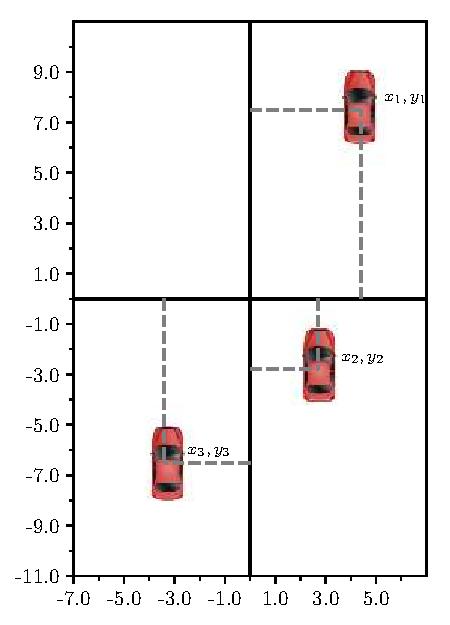
\includegraphics[width=0.35\textwidth]{../img/coordinates}
	
	List of features representation
\end{center}

\textbf{Requirements for function approximation}

\begin{enumerate}
	\item Permutation Invariance

\begin{align*}
\forall\tau \in \mathfrak{S}_N, \qquad &\pi(\cdot|(s_0, s_1,\dotsc,s_N)) = \\ &\pi(\cdot|(s_0, s_{\tau(1)},\dotsc,s_{\tau(N)}))
\end{align*}

\item Variable size

\end{enumerate}




\begin{center}
	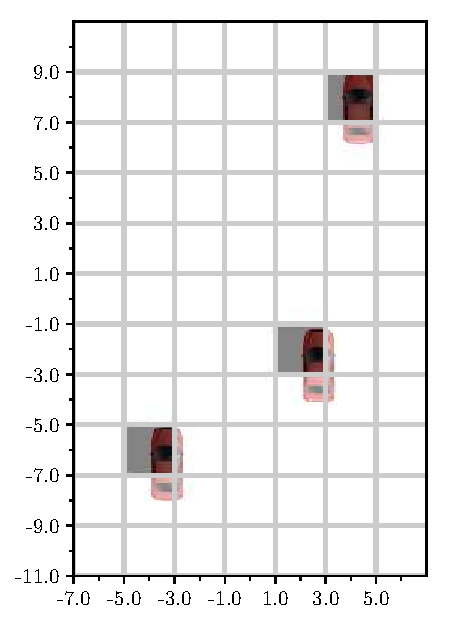
\includegraphics[width=0.35\textwidth]{../img/map}
	
	Occupancy grid representation
\end{center}

}


%----------------------------------------------------------------------------------------
%	Model Architecture
%----------------------------------------------------------------------------------------
\headerbox{Model Architecture}{name=archi,column=1,span=2}{

\textbf{Self-Attention}
\begin{equation}
\text{output}=\underbrace{\sigma\left(\frac{QK^T}{\sqrt{d_k}}\right)}_{\text{attention matrix}}V
\label{eq:selfattention}
\end{equation}


\begin{center}

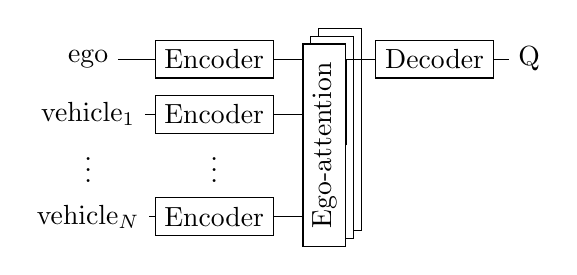
\begin{tikzpicture}
	\node(X1){ego};
	\node[below of=X1, node distance=0.7cm](X2){vehicle$_{1}$};
	\node[below of=X2, node distance=0.6cm](X3){$\vdots$};
	\node[below of=X3, node distance=0.7cm](X4){vehicle$_{N}$};
	
	\node[draw, right of=X1, node distance=1.6cm, rectangle](ENC1){Encoder};
	\node[draw, right of=X2, node distance=1.6cm, rectangle](ENC2){Encoder};
	\node[below of=ENC2, node distance=0.6cm](ENC3){$\vdots$};
	\node[draw, right of=X4, node distance=1.6cm, rectangle](ENC4){Encoder};
	
	\path (X1) edge (ENC1);
	\path (X2) edge (ENC2);
	\path (X4) edge (ENC4);
	
	
	\node[draw, rectangle, right of=ENC1, node distance=1.6cm, below=-0.4cm, fill=white](TRANS3){\rotatebox{90}{ Ego-attention }};
	\node[draw, rectangle, right of=ENC1, node distance=1.5cm, below=-0.3cm, fill=white](TRANS2){\rotatebox{90}{ Ego-attention }};
	\node[draw, rectangle, right of=ENC1, node distance=1.4cm, below=-0.2cm, fill=white](TRANS1){\rotatebox{90}{ Ego-attention }};
	
	\draw (ENC1.east) -| (TRANS1.west);
	\draw (ENC2.east) -| (TRANS1.west);
	\draw (ENC4.east) -| (TRANS1.west);
	
	
	\node[draw, right of=ENC1, node distance=2.8cm, rectangle](DEC1){Decoder};
	
	\draw (TRANS1.east) |- (DEC1.west);
	
	\node[right of=DEC1, node distance=1.2cm](Y1){Q};
	
	\draw (DEC1.east) -- (Y1.west);
\end{tikzpicture}
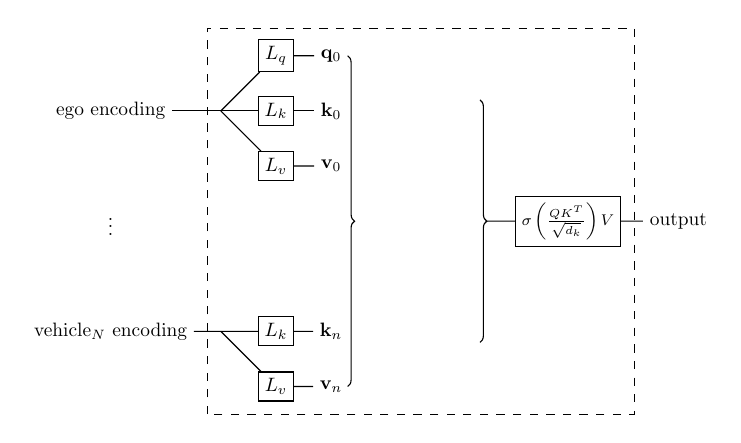
\begin{tikzpicture}[scale=0.7, every node/.style={scale=0.7}]
\node(X1){ego encoding};
\node[below of=X1, node distance=2cm](X2){$\vdots$};
\node[below of=X2, node distance=2cm](X3){vehicle$_{N}$ encoding};

\coordinate[right of= X1, node distance=2cm](X1b){};

\draw (X1) -- (X1b);

\node[draw, right of=X1b, node distance=1cm](LK1){$L_{k}$};
\node[draw, below of=LK1, node distance=1cm](LV1){$L_{v}$};
\node[draw, above of=LK1, node distance=1cm](LQ1){$L_{q}$};

\draw (X1b) -- (LQ1);
\draw (X1b) -- (LK1);
\draw (X1b) -- (LV1);


\node[right of=LQ1, node distance=1cm](Q1){$\mathbf{q}_0$};
\node[right of=LK1, node distance=1cm](K1){$\mathbf{k}_0$};
\node[right of=LV1, node distance=1cm](V1){$\mathbf{v}_0$};

\draw (LQ1) -- (Q1);
\draw (LK1) -- (K1);
\draw (LV1) -- (V1);

\coordinate[right of= X3, node distance=2cm](X3b){};

\draw (X3) -- (X3b);

\node[draw, right of=X3b, node distance=1cm](LK3){$L_{k}$};
\node[draw, below of=LK3, node distance=1cm](LV3){$L_{v}$};

\draw (X3b) -- (LK3);	
\draw (X3b) -- (LV3);

\node[right of=LK3, node distance=1cm](K3){$\mathbf{k}_{n}$};
\node[right of=LV3, node distance=1cm](V3){$\mathbf{v}_{n}$};

\draw (LK3) -- (K3);
\draw (LV3) -- (V3);

\coordinate[right of=Q1, node distance=0.3cm](TOP){};
\coordinate[right of=V3, node distance=0.3cm](BOT){};
\draw[decorate,decoration={brace}] (TOP) -- node[left=5pt]{} (BOT);

\node[right of=X2, text width=3cm, node distance=5.5cm](EQ){
};

\node[draw, right of=X2, node distance=8.3cm](EQ2){
	\footnotesize $\sigma\left(\frac{QK^T}{\sqrt{d_k}}\right)V$};

\coordinate[left of=EQ2, node distance=1.6cm, above=2.2cm](TOP2){};
\coordinate[left of=EQ2, node distance=1.5cm, below=0.0cm](MID2){};
\coordinate[left of=EQ2, node distance=1.6cm, below=2.2cm](BOT2){};
\draw[decorate,decoration={brace}] (TOP2) -- node[left=5pt]{} (BOT2);
\draw (MID2) -- (EQ2);

\node[right of=EQ2, node distance=2cm](OUT){output};
\draw (EQ2) -- (OUT);

\draw[draw=black, dashed] (1.75cm, -5.5cm) rectangle (9.5cm,1.5cm);
\end{tikzpicture}

\end{center}

}

%
%%----------------------------------------------------------------------------------------
%% Experiments
%%----------------------------------------------------------------------------------------
%
\headerbox{Experiments}{name=experiments,span=2,column=1,below=archi, above=bottom}{ 
\begin{center}
	\textbf{Agents}
	
	\begin{tabular}{lccc}
		\toprule
		Agent & \MLPL & \CNNG & \EgoAtt \\
		\midrule 
		Input sizes & [15, 7] & [11, 11, 7] & [1-15, 7] \\
		Layers sizes & [128, 128] &  \makecell[tc]{Convolutional layers: 3 \\ Kernel Size: 2 \\
			Stride: 2 \\ Head: [20]} & \makecell[tl]{Encoder: [64, 64] \\Attention: 2 heads, $d_k=32$ \\ Decoder: [64, 64]} \\
		Number of parameters & 3.0e4 & 3.2e4 & 3.4e4 \\
		Variable input size & No & No &  {Yes}  \\
		Permutation invariant & No & {Yes} &  {Yes} \\
		\bottomrule
	\end{tabular}
\end{center}

\begin{center}
	\textbf{Performances}
	
	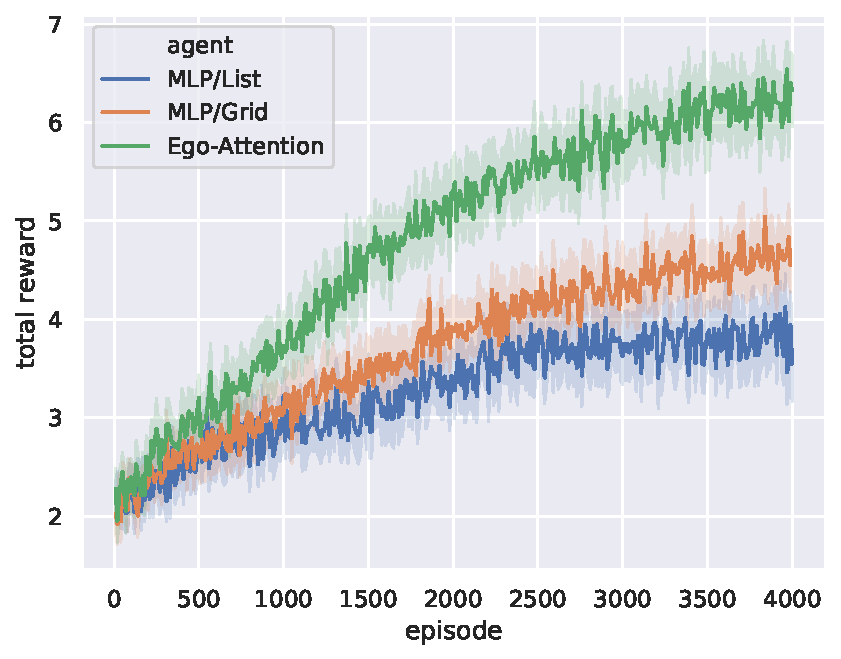
\includegraphics[width=0.32\linewidth]{../img/total_reward}
	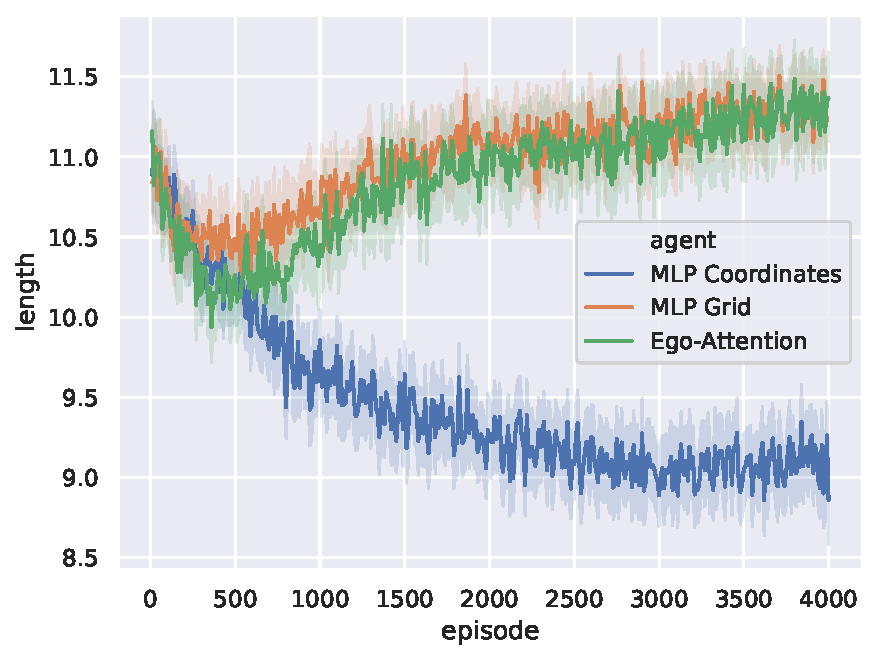
\includegraphics[width=0.32\linewidth]{../img/length}
	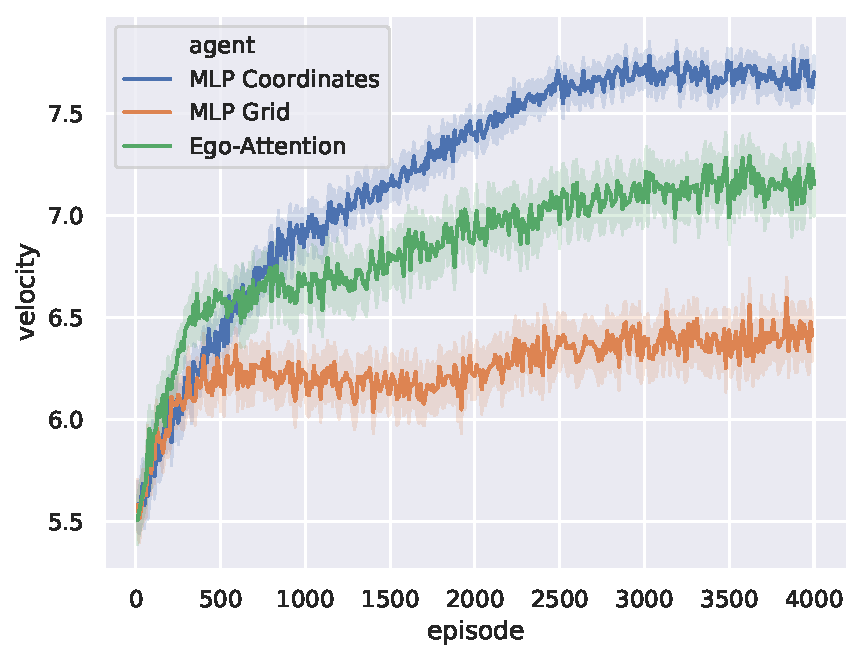
\includegraphics[width=0.32\linewidth]{../img/velocity}
\end{center}

\begin{center}
\textbf{Interpretation}

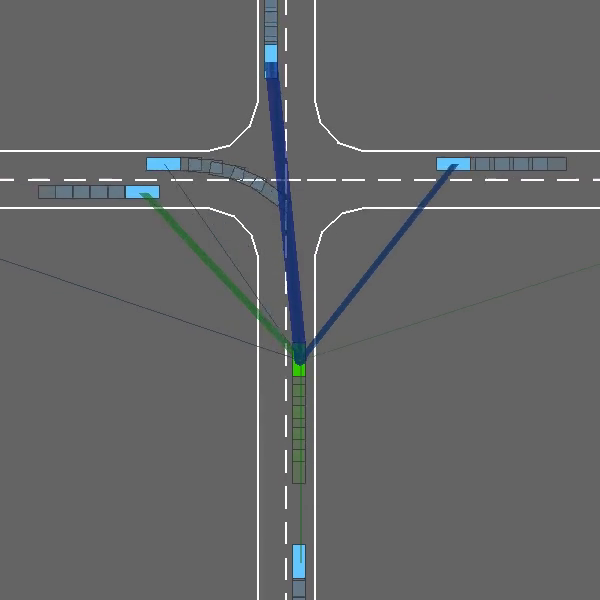
\includegraphics[width=0.26\linewidth]{../img/head_specialization}
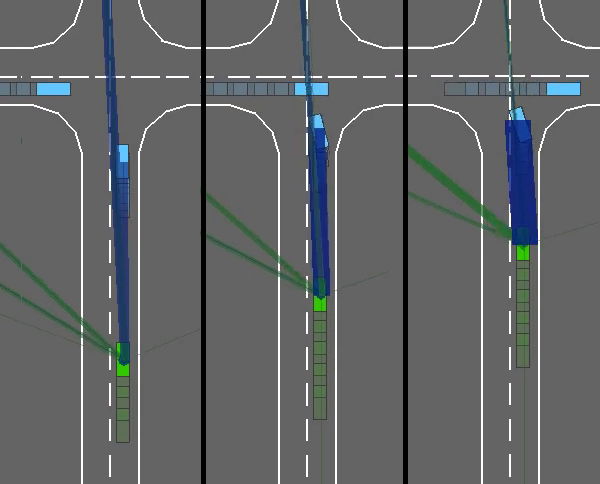
\includegraphics[width=0.28\linewidth]{../img/distances}
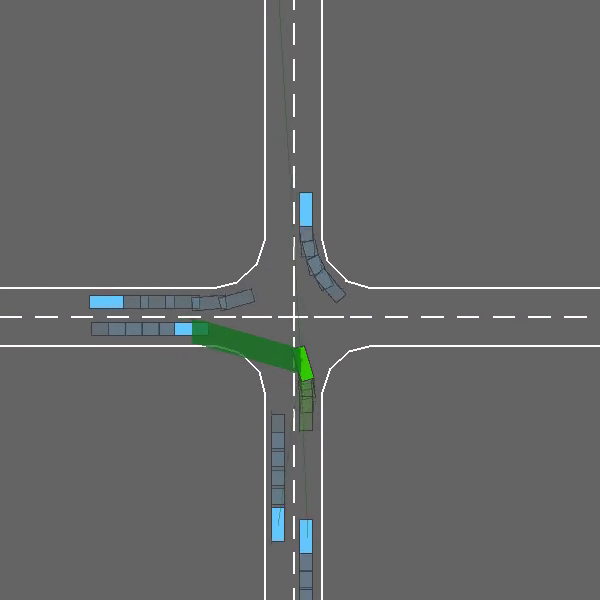
\includegraphics[width=0.21\linewidth]{../img/watch1}
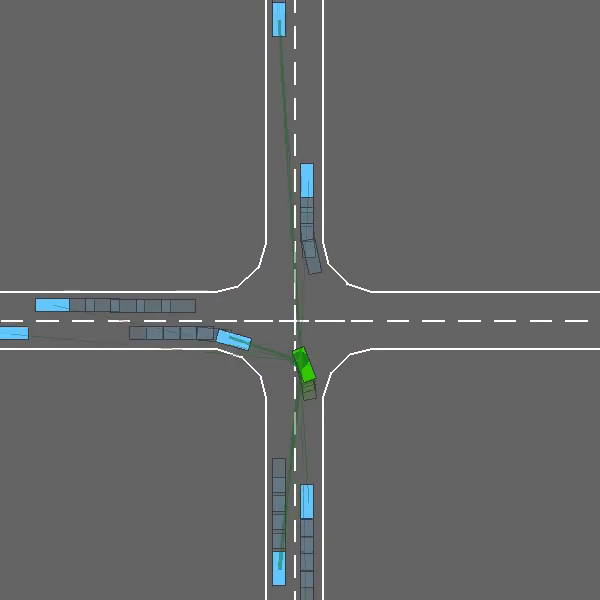
\includegraphics[width=0.21\linewidth]{../img/watch2}

Head specialisation \qquad\qquad\qquad Distance \qquad\qquad\qquad\qquad\qquad Sensitivity to uncertainty \qquad\qquad\qquad\qquad

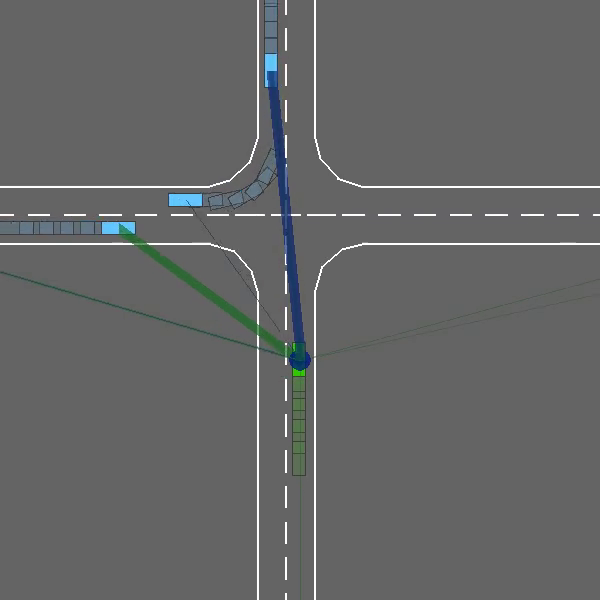
\includegraphics[width=.159\linewidth]{../img/episode1}
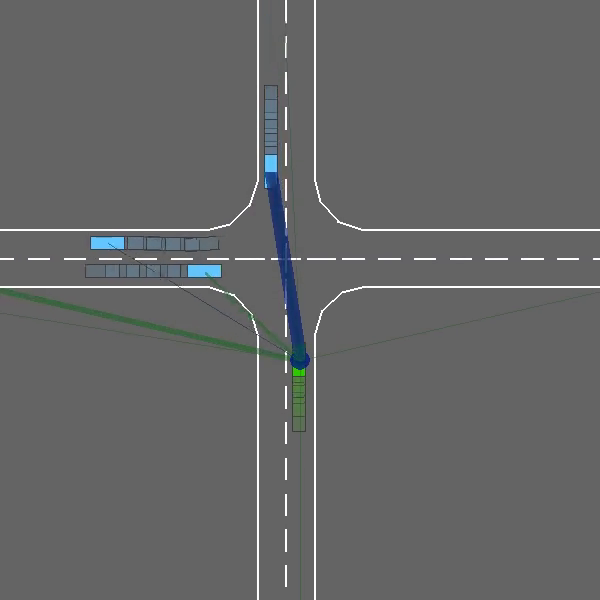
\includegraphics[width=.159\linewidth]{../img/episode2}
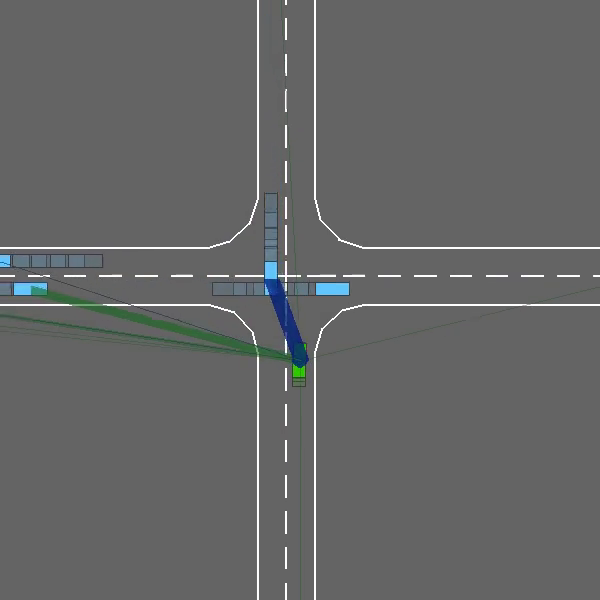
\includegraphics[width=.159\linewidth]{../img/episode3}
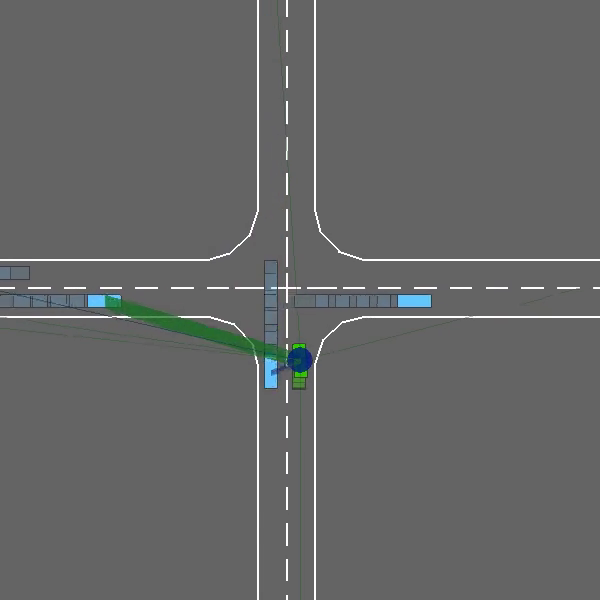
\includegraphics[width=.159\linewidth]{../img/episode4}
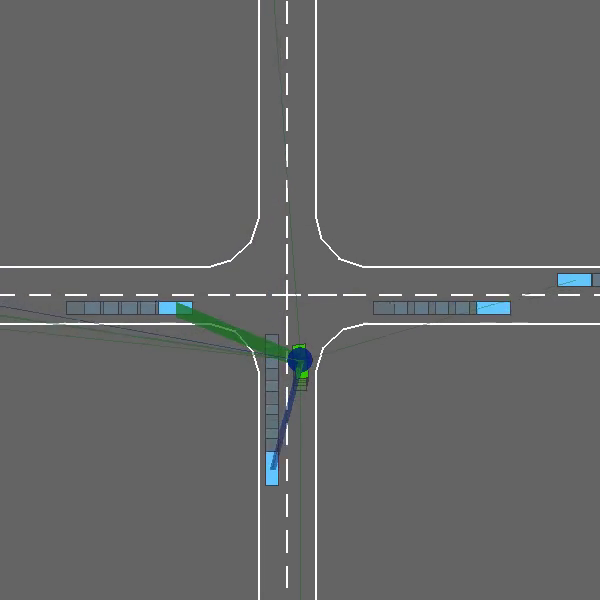
\includegraphics[width=.159\linewidth]{../img/episode5}
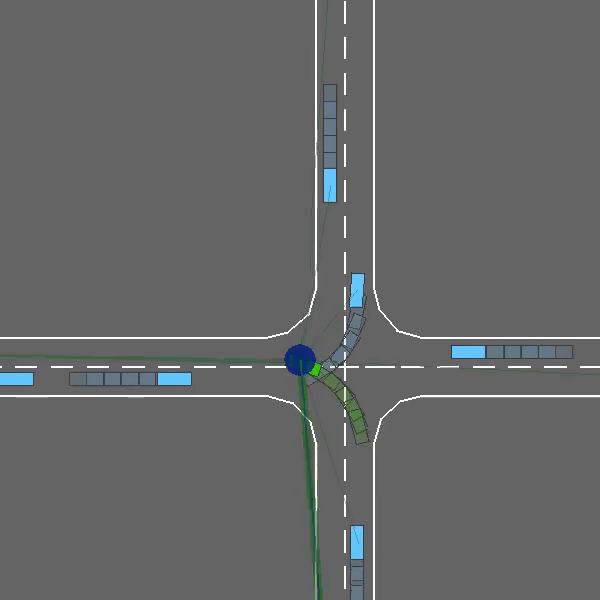
\includegraphics[width=.159\linewidth]{../img/episode6}

A full episode

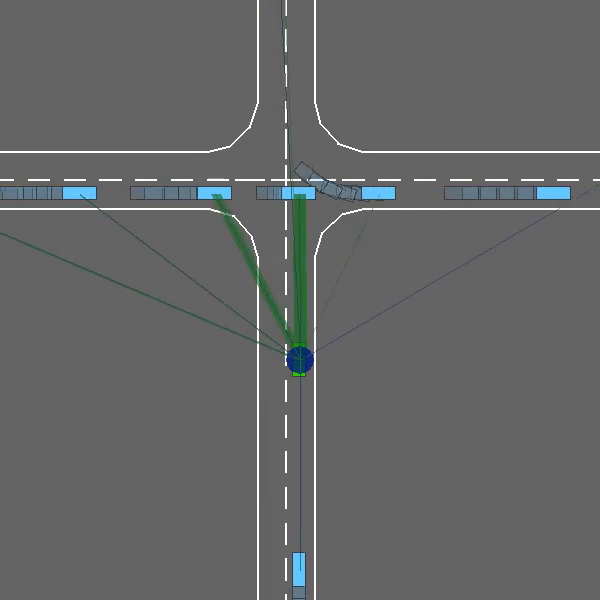
\includegraphics[width=0.2\linewidth]{../img/priority1}
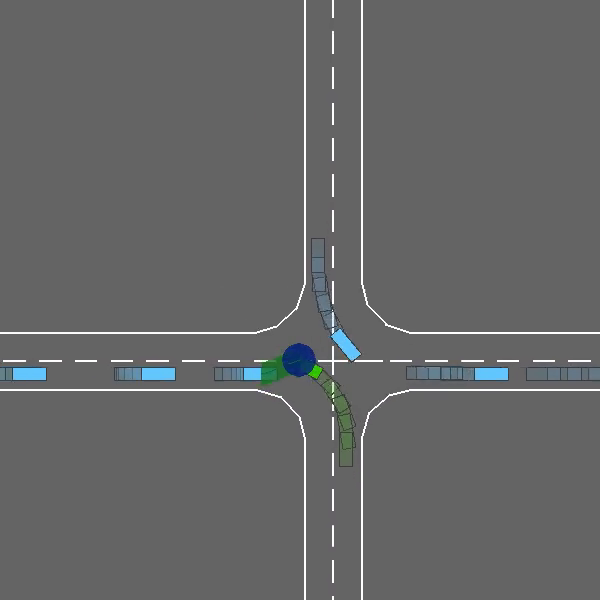
\includegraphics[width=0.2\linewidth]{../img/priority2}

Exploiting interaction patterns
\end{center}

}



%----------------------------------------------------------------------------------------
%	Acknowledgements
%----------------------------------------------------------------------------------------
\headerbox{Acknowledgements}{name=ack,column=0,span=1,below=setting}{
This work has been supported by CPER Nord-Pas de Calais/FEDER DATA Advanced data science and technologies 2015-2020, the French Ministry of Higher Education and Research, INRIA, and the French Agence Nationale de la Recherche (ANR).
}


%----------------------------------------------------------------------------------------
%	References
%----------------------------------------------------------------------------------------
\headerbox{References}{name=refs,column=0,span=1,below=ack, above=bottom}{
    {
    \AtNextBibliography{\footnotesize}
    \setlength{\bibitemsep}{3pt}
    \printbibliography[heading=none]
    }
}


\end{poster}

\end{document}


